% The Loop Economy: the 30-minute version (the 5-minute deck is ../slides.tex)
% Build: make   (pdflatex, two passes)
% Notes and timing: notes.md. Figures are TikZ, inline, so the deck is one file.
\documentclass[aspectratio=169,11pt]{beamer}
\usepackage[T1]{fontenc}
\usepackage{lmodern}
\usepackage{tgheros}
\renewcommand{\familydefault}{\sfdefault}
\usepackage{amsmath,amssymb}
\usepackage{booktabs}
\usepackage{array}
\usepackage{qrcode}
\usepackage{tikz}
\usetikzlibrary{arrows.meta,positioning,calc,fit,backgrounds,decorations.pathreplacing}

% --- one accent, one highlight, thin lines (as docs/talk/slides/figstyle.tex) ---
\definecolor{ink}{RGB}{34,34,34}
\definecolor{soft}{RGB}{105,105,105}
\definecolor{faint}{RGB}{222,222,222}
\definecolor{accent}{RGB}{0,95,115}
\definecolor{accentlight}{RGB}{214,232,236}
\definecolor{warn}{RGB}{196,84,40}
\definecolor{warnlight}{RGB}{247,226,216}
\tikzset{
  every picture/.style={color=ink, line width=0.5pt, font=\small},
  box/.style={draw=ink, rounded corners=2pt, fill=white, inner sep=4pt, minimum height=7mm, align=center},
  maker/.style={box, minimum width=17mm, font=\small\bfseries},
  cat/.style={box, inner sep=2.5pt, minimum height=5mm, font=\scriptsize},
  root/.style={box, fill=accentlight, draw=accent},
  bad/.style={box, fill=warnlight, draw=warn},
  flow/.style={-{Stealth[length=5pt,width=4pt]}, line width=0.6pt},
  sub/.style={-{Stealth[length=4pt,width=3.5pt]}, line width=0.5pt, color=soft},
  strong/.style={flow, color=accent, line width=0.9pt},
  lbl/.style={font=\footnotesize, text=ink, inner sep=1.5pt, fill=white},
  note/.style={font=\footnotesize, text=soft, align=center},
  rate/.style={font=\footnotesize, text=accent, inner sep=1pt, fill=white},
  person/.style={circle, draw=ink, fill=white, minimum size=5mm, inner sep=0pt},
}

% --- a quiet theme ----------------------------------------------------------
\usetheme{default}
\setbeamertemplate{navigation symbols}{}
\setbeamercolor{normal text}{fg=ink}
\setbeamercolor{structure}{fg=accent}
\setbeamercolor{frametitle}{fg=ink}
\setbeamercolor{alerted text}{fg=warn}
\setbeamerfont{frametitle}{size=\Large, series=\bfseries}
\setbeamertemplate{frametitle}{\vspace*{5mm}\insertframetitle\par\vspace*{0mm}}
\setbeamertemplate{itemize items}{\textcolor{accent}{\raisebox{0.3ex}{\rule{0.85ex}{0.85ex}}}}
\setbeamertemplate{itemize subitem}{\textcolor{soft}{--}}
\setlength{\leftmargini}{1.2em}
\setbeamersize{text margin left=10mm, text margin right=10mm}
% Every slide carries the repository and the project's page (devcon.txt;
% Peter, 2026-11-05). A frame inside a group may change either side, or
% add a centre.
\newcommand{\footleft}{github.com/petfold/loopmarket}
\newcommand{\footright}{loopmarket.eth.limo}
\newcommand{\footcentre}{}
\setbeamertemplate{footline}{%
  \leavevmode\hbox to \paperwidth{\hspace*{10mm}%
    \rlap{\footnotesize\color{soft}\footleft}\hfill
    {\footnotesize\color{ink}\footcentre}\hfill
    \llap{\footnotesize\color{soft}\footright\hspace{6mm}\insertframenumber}\hspace*{10mm}}%
  \vspace*{3.5mm}}

\newcommand{\sep}{\enspace\textperiodcentered\enspace}
\newcommand{\tick}{\textcolor{accent}{\checkmark}}
\newcommand{\todo}{\textcolor{soft}{$\circ$}}
\newcommand{\cross}{\textcolor{warn}{$\times$}}
\newcommand{\code}[1]{{\ttfamily #1}}
\newcommand{\qr}[2]{\qrcode[height=#1]{#2}}
\newcommand{\shade}[3]{\fcolorbox{#1}{#1}{\parbox{#2}{\raggedright #3}}}

\title{The Loop Economy}
\subtitle{A universal combinatorial marketplace\\ without a platform}
\author{Peter F\"oldi\'ak}
\date{November 2026}

\begin{document}
% ================================================================ 1 title
{\renewcommand{\footleft}{}
\begin{frame}
  \vspace*{6mm}
  \begin{columns}[c]
    \begin{column}{0.66\textwidth}
      {\fontsize{28}{32}\selectfont\bfseries\inserttitle\par}
      \vspace{3mm}
      {\large\insertsubtitle\par}
      \vspace{10mm}
      {\normalsize\insertauthor\quad{\color{accent}@petfold}\par}
      \vspace{1.5mm}
      {\small\color{soft}\insertdate\par}
      \vspace{8mm}
      {\footnotesize\color{soft}loopmarket\sep ontodag\sep factbond\sep on Swarm\par}
    \end{column}
    \begin{column}{0.30\textwidth}
      \centering
      \qr{31mm}{https://github.com/petfold/loopmarket}\par
      \vspace{2mm}
      {\footnotesize github.com/petfold/loopmarket\par}
    \end{column}
  \end{columns}
\end{frame}
}

% ---------------------------------------------------------------- part 1: the problem and the idea

% ================================================================ 2 problem
\begin{frame}{Most good trades never happen}
  \begin{columns}[c]
    \begin{column}{0.50\textwidth}
      \small
      \begin{itemize}\setlength{\itemsep}{2mm}
        \item Markets let strangers cooperate, voluntarily: a part of individual freedom.
        \item Online, that means \textbf{search}: shop after shop, each with its own catalogue, terms and checkout, and you never know you found the best deal.
        \item Or a \textbf{platform} that owns the index: it takes a cut, decides who is seen, and can delist anyone.
      \end{itemize}
      \vspace{3mm}
      {\color{accent}\bfseries Most mutually profitable trades fail on discovery, not on price: finding them costs more than they are worth.\par}
    \end{column}
    \begin{column}{0.48\textwidth}
      \centering
      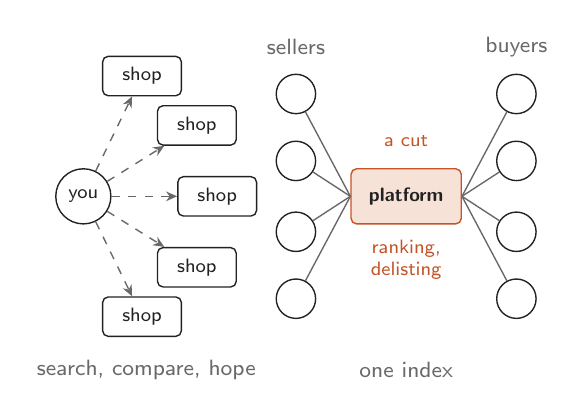
\begin{tikzpicture}[shop/.style={box, minimum width=10mm, minimum height=5mm, inner sep=1.5pt, font=\scriptsize}]
        % search: one buyer, many islands
        \node[person, minimum size=7mm, font=\scriptsize] (you) at (0,0) {you};
        \foreach \i/\a in {1/64,2/32,3/0,4/-32,5/-64} {
          \node[shop] (s\i) at (\a:17mm) {shop};
          \draw[sub, dashed] (you) -- (s\i);
        }
        \node[note] at (8mm,-22mm) {search, compare, hope};
        % platform: everyone through one company
        \begin{scope}[xshift=41mm]
          \node[bad, minimum width=14mm, font=\scriptsize\bfseries] (P) at (0,0) {platform};
          \foreach \i/\y in {1/13,2/4.5,3/-4.5,4/-13} {
            \node[person] (m\i) at (-14mm,\y mm) {};
            \node[person] (b\i) at (14mm,\y mm) {};
            \draw[soft] (m\i) -- (P.west); \draw[soft] (P.east) -- (b\i);
          }
          \node[font=\scriptsize, text=warn] at (0,7mm) {a cut};
          \node[font=\scriptsize, text=warn, align=center] at (0,-8mm) {ranking,\\ delisting};
          \node[note] at (-14mm,19mm) {sellers}; \node[note] at (14mm,19mm) {buyers}; \node[note] at (0,-22mm) {one index};
        \end{scope}
      \end{tikzpicture}
    \end{column}
  \end{columns}
\end{frame}
% ================================================================ 3 idea
\begin{frame}{Describe, don't search: solvers find the trade}
  \vspace{-2mm}
  \begin{columns}[T]
    \begin{column}{0.31\textwidth}
      \centering
      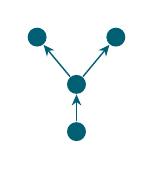
\begin{tikzpicture}[d/.style={circle, fill=accent, inner sep=0pt, minimum size=2.4mm}]
        \node[d] (a) at (-5mm,6mm) {}; \node[d] (b) at (5mm,6mm) {};
        \node[d] (c) at (0,0) {}; \node[d] (e) at (0,-6mm) {};
        \draw[sub, color=accent] (c) -- (a); \draw[sub, color=accent] (c) -- (b);
        \draw[sub, color=accent] (e) -- (c);
      \end{tikzpicture}\par
      \vspace{1.5mm}
      {\large\bfseries\color{accent}universal\par}\vspace{0.5mm}
    \end{column}
    \begin{column}{0.31\textwidth}
      \centering
      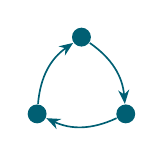
\begin{tikzpicture}[d/.style={circle, fill=accent, inner sep=0pt, minimum size=2.4mm}]
        \node[d] (a) at (90:6.5mm) {}; \node[d] (b) at (210:6.5mm) {}; \node[d] (c) at (330:6.5mm) {};
        \draw[flow, color=accent] (a) to[bend left=25] (c);
        \draw[flow, color=accent] (c) to[bend left=25] (b);
        \draw[flow, color=accent] (b) to[bend left=25] (a);
      \end{tikzpicture}\par
      \vspace{1.5mm}
      {\large\bfseries\color{accent}combinatorial\par}\vspace{0.5mm}
    \end{column}
    \begin{column}{0.31\textwidth}
      \centering
      
\begin{tikzpicture}[d/.style={circle, fill=accent, inner sep=0pt, minimum size=2.4mm}]
        \foreach \i in {0,...,5} { \node[d] (p\i) at (\i*60:7mm) {}; }
        \foreach \i/\j in {0/1,1/2,2/3,3/4,4/5,5/0,0/2,1/4,3/5} { \draw[color=accent] (p\i) -- (p\j); }
      \end{tikzpicture}\par
      \vspace{1.5mm}
      {\large\bfseries\color{accent}permissionless\par}\vspace{0.5mm}
    \end{column}
  \end{columns}
  \vspace{1mm}
  \begin{columns}[T]\small
    \begin{column}{0.31\textwidth}
      Anything that can be described exactly: rides, repairs, parcels, storage, energy, care\dots\ and money, as one more offer. Not only tokens.
    \end{column}
    \begin{column}{0.31\textwidth}
      Many offers combine into one trade: loops of three, five, ten makers; a courier's leg composed into a delivery. Algorithms do the searching.
    \end{column}
    \begin{column}{0.31\textwidth}
      Every maker keeps their own offer book on Swarm. No platform, no protocol fee, nobody who can delist you.
    \end{column}
  \end{columns}
  \vspace{4mm}
  \begin{center}
    \shade{accentlight}{0.95\textwidth}{\centering\small
      CoW Protocol finds coincidences of wants among tokens, to beat the AMM price.\\
      \textbf{loopmarket finds them where there is no AMM to beat.}}
  \end{center}
\end{frame}

% ---------------------------------------------------------------- part 2: offers, loops and circulations

% ================================================================ 4 offer
\begin{frame}{One offer form for everything}
  \vspace{-1mm}
  \centering
  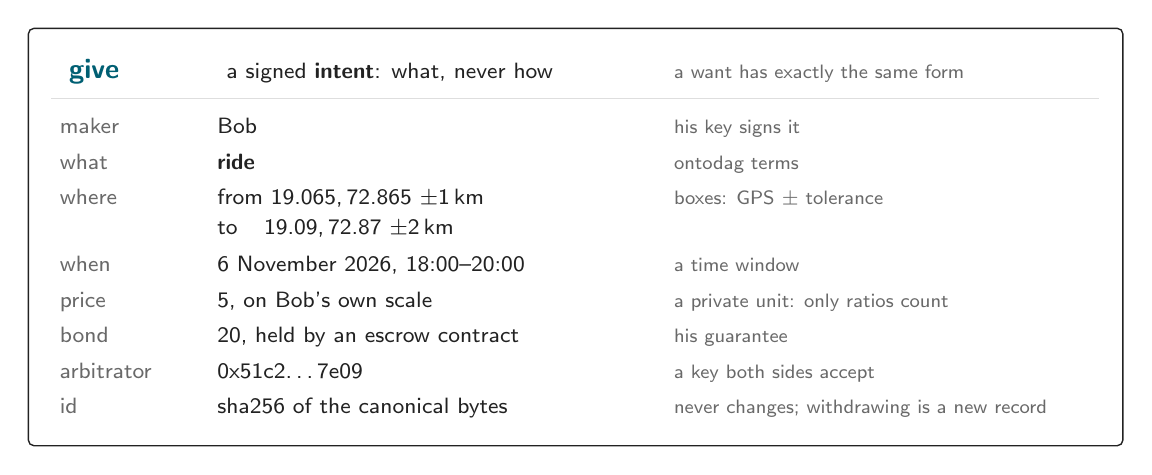
\begin{tikzpicture}[k/.style={anchor=base west, font=\footnotesize, text=soft, inner sep=0pt},
                      v/.style={anchor=base west, font=\footnotesize, inner sep=0pt},
                      c/.style={anchor=base west, font=\scriptsize, text=soft, inner sep=0pt}]
    \node[box, minimum width=139mm, minimum height=53mm, anchor=north west] at (0,0) {};
    \node[anchor=base west, font=\normalsize\bfseries, text=accent] at (4mm,-6.5mm) {give};
    \node[anchor=base west, font=\footnotesize] at (24mm,-6.5mm) {a signed \textbf{intent}: what, never how};
    \node[c] at (82mm,-6.5mm) {a want has exactly the same form};
    \draw[faint] (3mm,-9mm) -- (136mm,-9mm);
    \foreach \y/\key/\val/\com in {
        -13.5/maker/{Bob}/{his key signs it},
        -18/what/{\textbf{ride}}/{ontodag terms},
        -22.5/where/{from 19.065,\,72.865 $\pm$1\,km}/{boxes: GPS $\pm$ tolerance},
        -26.3/{}/{to\phantom{m} 19.09,\,72.87 $\pm$2\,km}/{},
        -31/when/{6 November 2026, 18:00--20:00}/{a time window},
        -35.5/price/{5, on Bob's own scale}/{a private unit: only ratios count},
        -40/bond/{20, held by an escrow contract}/{his guarantee},
        -44.5/arbitrator/{0x51c2\dots7e09}/{a key both sides accept},
        -49/id/{sha256 of the canonical bytes}/{never changes; withdrawing is a new record}} {
      \node[k] at (4mm,\y mm) {\key};
      \node[v] at (24mm,\y mm) {\val};
      \node[c] at (82mm,\y mm) {\com};
    }
  \end{tikzpicture}\par
  \vspace{2.5mm}
  \raggedright
  {\small Own scale: $k$ gives and $m$ wants need $k+m$ prices, not $k\times m$ exchange rates.\par}
  \vspace{1mm}
  {\scriptsize\ttfamily\color{soft}\$ loop give ride \textquotesingle{}from(Jio)\textquotesingle{} \textquotesingle{}to(BOM)\textquotesingle{} \textquotesingle{}time(2026-11-06T12:30:00Z..2026-11-06T14:30:00Z)\textquotesingle{} 5\par}
\end{frame}
\begin{frame}{Why a personal scale}
  \centering
  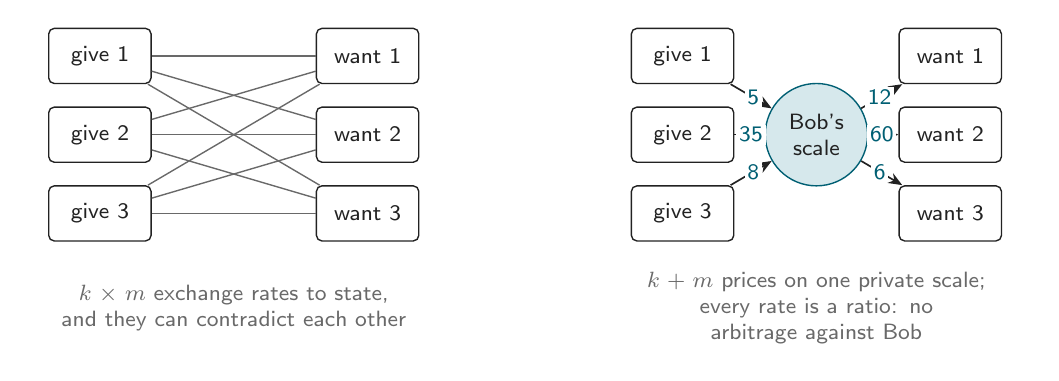
\begin{tikzpicture}[item/.style={box, inner sep=2.5pt, minimum width=13mm, font=\footnotesize}]
    \begin{scope}
      \foreach \i/\y in {1/10,2/0,3/-10} { \node[item] (g\i) at (0,\y mm) {give \i}; }
      \foreach \j/\y in {1/10,2/0,3/-10} { \node[item] (w\j) at (34mm,\y mm) {want \j}; }
      \foreach \i in {1,2,3} \foreach \j in {1,2,3} { \draw[soft] (g\i) -- (w\j); }
      \node[note, text width=50mm] at (17mm,-22mm) {$k \times m$ exchange rates to state,\\ and they can contradict each other};
    \end{scope}
    \begin{scope}[xshift=74mm]
      \node[root, circle, inner sep=1pt, minimum size=13mm, font=\footnotesize, align=center] (S) at (17mm,0) {Bob's\\ scale};
      \foreach \i/\y/\p in {1/10/5,2/0/35,3/-10/8} { \node[item] (g\i) at (0,\y mm) {give \i}; \draw[flow] (g\i) -- node[rate, pos=0.55] {\p} (S); }
      \foreach \j/\y/\p in {1/10/12,2/0/60,3/-10/6} { \node[item] (w\j) at (34mm,\y mm) {want \j}; \draw[flow] (S) -- node[rate, pos=0.45] {\p} (w\j); }
      \node[note, text width=52mm] at (17mm,-22mm) {$k + m$ prices on one private scale;\\ every rate is a ratio: no arbitrage against Bob};
    \end{scope}
  \end{tikzpicture}\par
  \vspace{5mm}
  \raggedright
  {\small The scale is bookkeeping, a personal numeraire: nothing is issued, held or transferred. Only ratios leave the maker, and round a loop the scales cancel. A batch is scored by the sum of the logs of its loops' surplus factors, so no common unit is ever needed.\par}
\end{frame}
% ================================================================ 5 loops
\begin{frame}{Loops: the trade nobody could find}
  \vspace{-1mm}
  \begin{columns}[T]
    \begin{column}{0.42\textwidth}
      \centering
      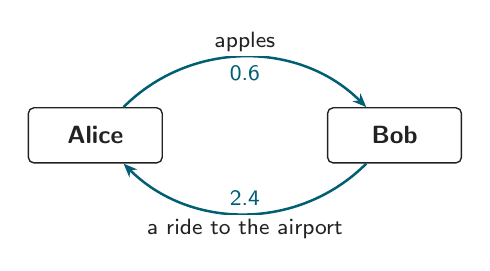
\begin{tikzpicture}
        \node[maker] (A) at (0,0) {Alice};
        \node[maker] (B) at (38mm,0) {Bob};
        \draw[strong] (A) to[bend left=45] node[lbl, above] {apples} node[rate, below=0.6mm] {0.6} (B);
        \draw[strong] (B) to[bend left=45] node[lbl, below] {a ride to the airport} node[rate, above=0.6mm] {2.4} (A);
      \end{tikzpicture}\par
      \vspace{1.5mm}
      {\small\color{accent}$\prod r = 0.6\times 2.4 = 1.44 > 1$\par}
      \vspace{1mm}
      {\small Barter needs a \emph{double coincidence of wants}, which is rare.\par}
    \end{column}
    \begin{column}{0.54\textwidth}
      \centering
      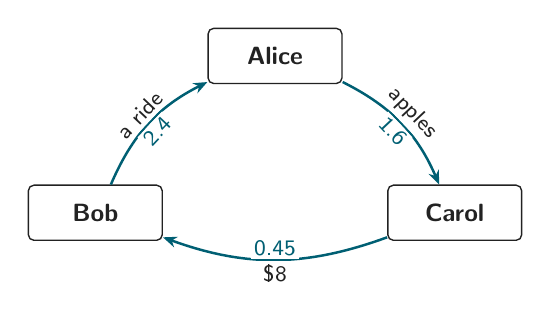
\begin{tikzpicture}
        \node[maker] (A) at (90:12.5mm) {Alice};
        \node[maker] (C) at (-18:24mm) {Carol};
        \node[maker] (B) at (198:24mm) {Bob};
        \draw[strong] (A) to[bend left=20] node[lbl, sloped, above] {apples} node[rate, sloped, below] {1.6} (C);
        \draw[strong] (C) to[bend left=20] node[lbl, below] {\$8} node[rate, above] {0.45} (B);
        \draw[strong] (B) to[bend left=20] node[lbl, sloped, above] {a ride} node[rate, sloped, below] {2.4} (A);
      \end{tikzpicture}\par
      \vspace{1mm}
      {\small\color{accent}$\prod r = 1.6\times 0.45\times 2.4 = 1.728 > 1$\par}
      \vspace{1mm}
      {\small Bob wants money, not apples. No pair can trade, yet the loop clears: money is one more leg.\par}
    \end{column}
  \end{columns}
  \vspace{2mm}
  \shade{accentlight}{0.975\textwidth}{\small
    A leg's rate $r$ is the wanter's price over the giver's, each on their own scale. $\prod r>1$ is a \textbf{negative cycle} under $-\log r$: Bellman--Ford finds it, as in DEX arbitrage, and the makers keep the surplus.}
\end{frame}

\begin{frame}{A loop of five: no pair, no three can trade}
  \centering
  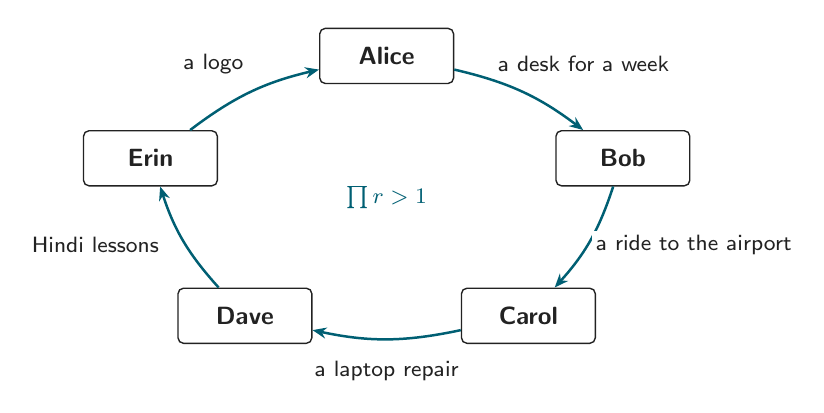
\begin{tikzpicture}[x=1mm,y=1mm]
    \node[maker] (A) at (0,18) {Alice};
    \node[maker] (B) at (30,5) {Bob};
    \node[maker] (C) at (18,-15) {Carol};
    \node[maker] (D) at (-18,-15) {Dave};
    \node[maker] (E) at (-30,5) {Erin};
    \draw[strong] (A) to[bend left=12] (B);
    \draw[strong] (B) to[bend left=12] (C);
    \draw[strong] (C) to[bend left=12] (D);
    \draw[strong] (D) to[bend left=12] (E);
    \draw[strong] (E) to[bend left=12] (A);
    \node[lbl] at (25,17) {a desk for a week};
    \node[lbl] at (39,-6) {a ride to the airport};
    \node[lbl] at (0,-22) {a laptop repair};
    \node[lbl] at (-37,-6) {Hindi lessons};
    \node[lbl] at (-22,17) {a logo};
    \node[font=\footnotesize, text=accent] at (0,0) {$\prod r>1$};
  \end{tikzpicture}\par
  \vspace{4mm}
  \raggedright
  {\small Each wants what only the one before has: Bob a desk, Carol a ride, Dave a repair, Erin lessons, Alice a logo. Nobody finds this by searching; for a solver it is one more cycle in the graph of matches. Clearing checks all five legs, and commits them together or not at all.\par}
\end{frame}


\begin{frame}{A profitable loop is a negative cycle}
  \begin{columns}[T]
    \begin{column}{0.48\textwidth}
      \centering
      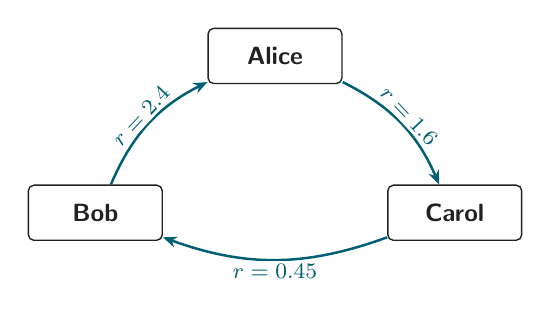
\begin{tikzpicture}
        \node[maker] (A) at (90:12.5mm) {Alice};
        \node[maker] (C) at (-18:24mm) {Carol};
        \node[maker] (B) at (198:24mm) {Bob};
        \draw[strong] (A) to[bend left=20] node[rate, sloped, above] {$r=1.6$} (C);
        \draw[strong] (C) to[bend left=20] node[rate, below] {$r=0.45$} (B);
        \draw[strong] (B) to[bend left=20] node[rate, sloped, above] {$r=2.4$} (A);
      \end{tikzpicture}\par
      \vspace{2mm}
      {\small $\prod r = 1.6\times 0.45\times 2.4 = 1.728 > 1$\par}
    \end{column}
    \begin{column}{0.48\textwidth}
      \centering
      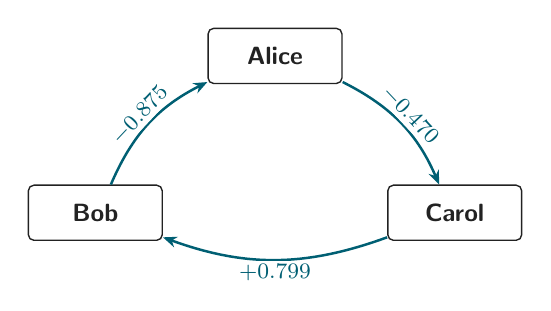
\begin{tikzpicture}
        \node[maker] (A) at (90:12.5mm) {Alice};
        \node[maker] (C) at (-18:24mm) {Carol};
        \node[maker] (B) at (198:24mm) {Bob};
        \draw[strong] (A) to[bend left=20] node[rate, sloped, above] {$-0.470$} (C);
        \draw[strong] (C) to[bend left=20] node[rate, below] {$+0.799$} (B);
        \draw[strong] (B) to[bend left=20] node[rate, sloped, above] {$-0.875$} (A);
      \end{tikzpicture}\par
      \vspace{2mm}
      {\small $\sum(-\log r) = -0.547 < 0$\par}
    \end{column}
  \end{columns}
  \vspace{3mm}
  \small
  \begin{itemize}\setlength{\itemsep}{1.2mm}
    \item Weigh each leg by $-\log r$: a loop with $\prod r>1$ becomes a cycle whose weights sum below zero, which Bellman--Ford finds in $O(V\!\cdot\!E)$: the standard arbitrage detector.
    \item The baseline search is deterministic (U6) and may round; clearing re-checks the product in exact rationals (U9), so rounding never clears a loop.
  \end{itemize}
\end{frame}


\begin{frame}{Many candidate loops, one offer: selection}
  \centering
  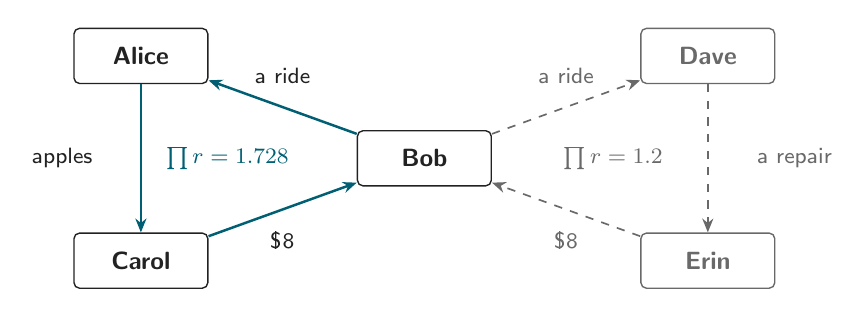
\begin{tikzpicture}[x=1mm,y=1mm]
    \node[maker] (Bo) at (0,0) {Bob};
    \node[maker] (Al) at (-36,13) {Alice};
    \node[maker] (Ca) at (-36,-13) {Carol};
    \node[maker, draw=soft, text=soft] (Da) at (36,13) {Dave};
    \node[maker, draw=soft, text=soft] (Er) at (36,-13) {Erin};
    \draw[strong] (Bo) -- (Al);
    \draw[strong] (Al) -- (Ca);
    \draw[strong] (Ca) -- (Bo);
    \draw[flow, soft, dashed] (Bo) -- (Da);
    \draw[flow, soft, dashed] (Da) -- (Er);
    \draw[flow, soft, dashed] (Er) -- (Bo);
    \node[lbl] at (-18,10.5) {a ride};
    \node[lbl] at (-46,0) {apples};
    \node[lbl] at (-18,-10.5) {\$8};
    \node[lbl, text=soft] at (18,10.5) {a ride};
    \node[lbl, text=soft] at (47,0) {a repair};
    \node[lbl, text=soft] at (18,-10.5) {\$8};
    \node[font=\footnotesize, text=accent] at (-25,0) {$\prod r=1.728$};
    \node[font=\footnotesize, text=soft] at (24,0) {$\prod r=1.2$};
  \end{tikzpicture}\par
  \vspace{3mm}
  \raggedright
  \small
  \begin{itemize}\setlength{\itemsep}{1.2mm}
    \item Bob has one ride and one want. Both loops need them, so at most one of the two can clear.
    \item Selection packs the candidates: the set of loops worth most within every offer's capacity, scored by $\sum \log\prod r$, a number with no unit.
    \item Exact branch and bound while the set is small, a deterministic greedy beyond it, and one total order for ties: every replica picks the same set.
  \end{itemize}
\end{frame}


\begin{frame}{One want, many gives: a circulation}
  \centering
  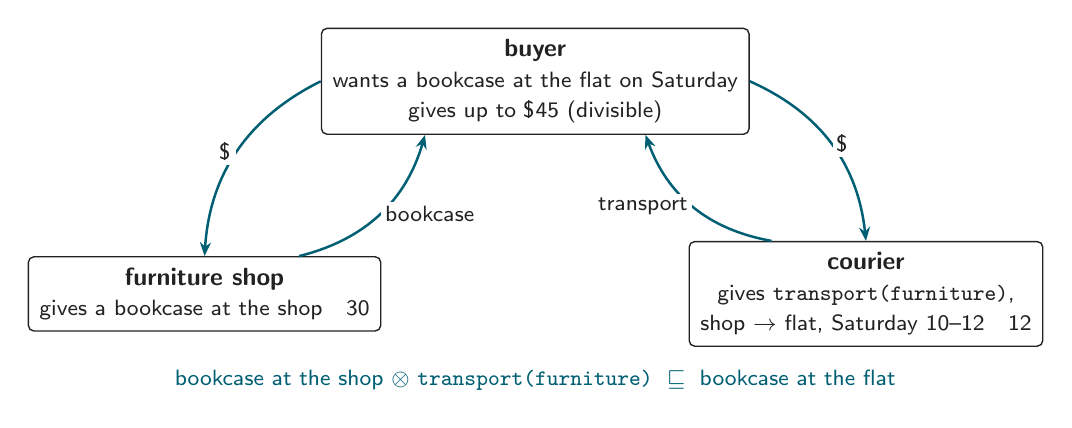
\begin{tikzpicture}
    \node[maker, align=center, font=\small\bfseries] (T) at (0,0) {buyer\\{\footnotesize\mdseries wants a bookcase at the flat on Saturday}\\{\footnotesize\mdseries gives up to \$45 (divisible)}};
    \node[maker, align=center, font=\small\bfseries] (S) at (-42mm,-27mm) {furniture shop\\{\footnotesize\mdseries gives a bookcase at the shop\quad 30}};
    \node[maker, align=center, font=\small\bfseries] (C) at (42mm,-27mm) {courier\\{\footnotesize\mdseries gives \texttt{transport(furniture)},}\\{\footnotesize\mdseries shop $\to$ flat, Saturday 10--12\quad 12}};
    \draw[strong] (T.west) to[bend right=30] node[lbl, left] {\$} (S.north);
    \draw[strong] (T.east) to[bend left=30] node[lbl, right] {\$} (C.north);
    \draw[strong] ($(S.north)+(12mm,0)$) to[bend right=30] node[lbl, right] {bookcase} ($(T.south)+(-14mm,0)$);
    \draw[strong] ($(C.north)+(-12mm,0)$) to[bend left=30] node[lbl, left] {transport} ($(T.south)+(14mm,0)$);
    \node[note, text=accent] at (0,-38mm) {bookcase at the shop $\otimes$ \texttt{transport(furniture)} $\;\sqsubseteq\;$ bookcase at the flat};
  \end{tikzpicture}\par
  \vspace{2mm}
  \raggedright
  {\small A circulation, not a cycle: every maker gives and receives, and nets to zero on their own scale. The \emph{one} want holds the conjunction, so it clears all or nothing, and clearing splits the one payment. A bookcase is furniture; a piano is not.\par}
\end{frame}


\begin{frame}{Quantities: aggregation and capacity}
  \begin{columns}[T]
    \begin{column}{0.48\textwidth}
      \centering
      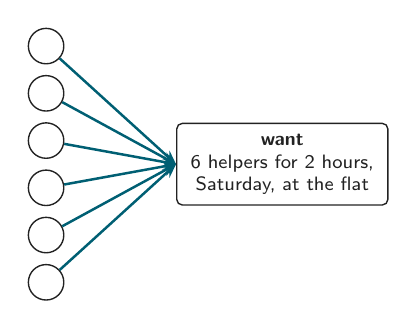
\begin{tikzpicture}[x=1mm,y=1mm]
        \node[box, text width=24mm, font=\scriptsize] (W) at (30,0) {\textbf{want}\\ 6 helpers for 2 hours, Saturday, at the flat};
        \foreach \i/\y in {1/15,2/9,3/3,4/-3,5/-9,6/-15} {
          \node[person, minimum size=4.5mm] (p\i) at (0,\y) {};
          \draw[strong] (p\i) -- (W.west);
        }
      \end{tikzpicture}\par
      \vspace{3mm}
      {\small\textbf{Aggregation.} Six neighbours each give one helper. The want takes all six or none, and its one payment splits six ways.\par}
    \end{column}
    \begin{column}{0.48\textwidth}
      \centering
      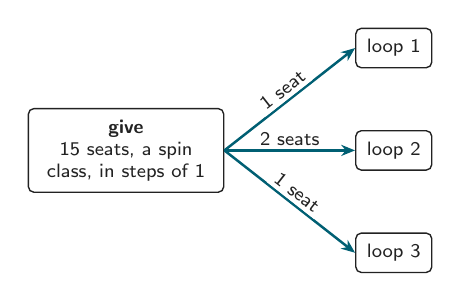
\begin{tikzpicture}[x=1mm,y=1mm]
        \node[box, text width=22mm, font=\scriptsize] (G) at (0,0) {\textbf{give}\\ 15 seats, a spin class, in steps of 1};
        \foreach \i/\y/\q in {1/13/1 seat,2/0/2 seats,3/-13/1 seat} {
          \node[box, font=\scriptsize, minimum height=5mm] (L\i) at (34,\y) {loop \i};
          \draw[strong] (G.east) -- node[lbl, font=\scriptsize, above, sloped] {\q} (L\i.west);
        }
      \end{tikzpicture}\par
      \vspace{3mm}
      {\small\textbf{Capacity.} Each loop takes what its want asks; the fills never sum past 15 (U11). A floor, \code{8seat..15seat:1}, runs only for at least eight in one loop.\par}
    \end{column}
  \end{columns}
\end{frame}


\begin{frame}{Parts: a want of several things, all or nothing}
  \centering
  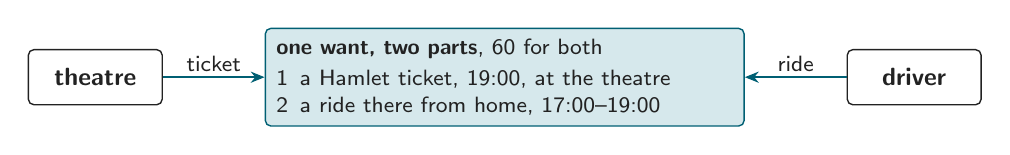
\begin{tikzpicture}[x=1mm,y=1mm]
    \node[box, text width=58mm, align=left, font=\footnotesize, fill=accentlight, draw=accent] (W) at (0,0) {\textbf{one want, two parts}, 60 for both\\[0.6mm] 1\enspace a Hamlet ticket, 19:00, at the theatre\\ 2\enspace a ride there from home, 17:00--19:00};
    \node[maker] (Th) at (-52,0) {theatre};
    \node[maker] (Dr) at (52,0) {driver};
    \draw[strong] (Th) -- node[lbl, above] {ticket} (W);
    \draw[strong] (Dr) -- node[lbl, above] {ride} (W);
  \end{tikzpicture}\par
  \vspace{4mm}
  \raggedright
  {\scriptsize\ttfamily\color{soft}\$ loop want theatre-ticket hamlet venue + ride \textquotesingle{}from(home)\textquotesingle{} \textquotesingle{}to(venue)\textquotesingle{} 60\par}
  \vspace{3mm}
  \small
  \begin{itemize}\setlength{\itemsep}{1.2mm}
    \item The ticket is worthless without the ride, and the ride without the ticket. Only you care, so the coupling lives in your want: its parts clear together or not at all.
    \item You price the bundle once; clearing splits it across the gives.
    \item Bundles live only on the want side: no give is ever conditional on another give.
  \end{itemize}
\end{frame}


\begin{frame}{The object: a circulation on a hypergraph}
  \begin{columns}[c]
    \begin{column}{0.36\textwidth}
      \centering
      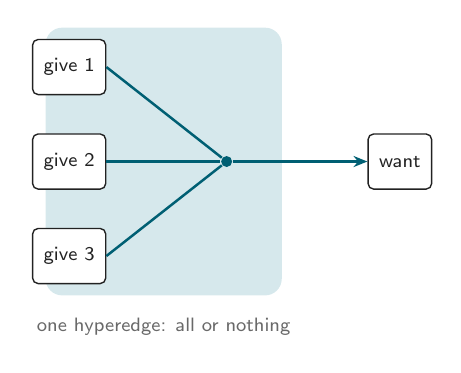
\begin{tikzpicture}[x=1mm,y=1mm]
        \fill[accentlight, rounded corners=6pt] (-3,-17) rectangle (27,17);
        \node[box, font=\scriptsize] (g1) at (0,12) {give 1};
        \node[box, font=\scriptsize] (g2) at (0,0) {give 2};
        \node[box, font=\scriptsize] (g3) at (0,-12) {give 3};
        \node[circle, fill=accent, inner sep=1.4pt] (j) at (20,0) {};
        \node[box, font=\scriptsize] (w) at (42,0) {want};
        \foreach \g in {g1,g2,g3} { \draw[color=accent, line width=0.9pt] (\g.east) -- (j); }
        \draw[strong] (j) -- (w);
        \node[note, font=\scriptsize] at (12,-21) {one hyperedge: all or nothing};
      \end{tikzpicture}
    \end{column}
    \begin{column}{0.62\textwidth}
      \small
      \begin{itemize}\setlength{\itemsep}{1.6mm}
        \item A leg is an edge between makers. A composed or aggregated leg is a \textbf{hyperedge}: several gives, one want, one flow, filled together or not at all.
        \item A cleared set is a \textbf{circulation}: at every maker, value in equals value out, on that maker's own scale. A loop is its smallest case.
        \item Clearing prices are \textbf{node potentials}: each maker's scale is one. At those prices the rates round every cycle multiply to 1: Kirchhoff's voltage law, in logs.
        \item So checking a proposal is a potential check, linear in the number of legs: something an on-chain verifier can afford.
      \end{itemize}
    \end{column}
  \end{columns}
\end{frame}


% ---------------------------------------------------------------- part 3: OntoDAG


{\renewcommand{\footleft}{github.com/petfold/ontodag}\renewcommand{\footright}{ontodag.eth.limo}

\begin{frame}{OntoDAG: categories form a DAG}
  \begin{columns}[T]
    \begin{column}{0.56\textwidth}
      \centering
      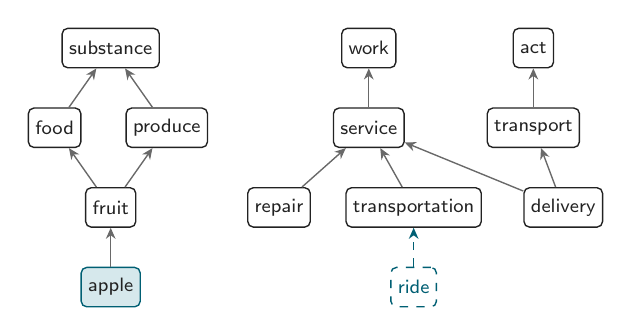
\begin{tikzpicture}[x=0.95mm, y=0.92mm]
        \node[cat] (substance) at (7.5,33) {substance};
        \node[cat] (work) at (42,33) {work};
        \node[cat] (act) at (64,33) {act};
        \node[cat] (food) at (0,22) {food};
        \node[cat] (produce) at (15,22) {produce};
        \node[cat] (service) at (42,22) {service};
        \node[cat] (transport) at (64,22) {transport};
        \node[cat] (fruit) at (7.5,11) {fruit};
        \node[cat] (repair) at (30,11) {repair};
        \node[cat] (transportation) at (48,11) {transportation};
        \node[cat] (delivery) at (68,11) {delivery};
        \node[cat, fill=accentlight, draw=accent] (apple) at (7.5,0) {apple};
        \node[cat, draw=accent, dashed, text=accent] (ride) at (48,0) {ride};
        \foreach \a/\b in {food/substance, produce/substance, fruit/food, fruit/produce, apple/fruit,
                           service/work, transport/act, repair/service, transportation/service,
                           delivery/service, delivery/transport} { \draw[sub] (\a) -- (\b); }
        \draw[sub, color=accent, dashed] (ride) -- (transportation);
      \end{tikzpicture}\par
      \vspace{1mm}
      {\tiny\color{soft}edges from ontodag's core pack (a selection); \textcolor{accent}{ride} is added with \code{put}\par}

    \end{column}
    \begin{column}{0.42\textwidth}
      \small
      \begin{itemize}\setlength{\itemsep}{2mm}
        \item \textbf{One relation, \emph{fits within}.} An arrow points to the wider category; everything below a category is a special case of it.
        \item \textbf{Several parents are normal.} An apple is food \emph{and} produce; a jigsaw is a saw \emph{and} a power tool; a delivery is a service \emph{and} a transport. No folder has to be chosen.
        \item \textbf{Keep no link you can infer.} The stored graph is minimal, so equal content gives an equal graph.
      \end{itemize}
    \end{column}
  \end{columns}
\end{frame}

\begin{frame}{put and get: a query is an intersection of cones}
  \begin{columns}[T]
    \begin{column}{0.52\textwidth}
      {\scriptsize\ttfamily
        \textcolor{soft}{\$} odag put Flight; odag put Japan\\[0.4mm]
        \textcolor{soft}{\$} odag put Hotel\\[0.4mm]
        \textcolor{soft}{\$} odag put JAL-123 Flight Japan\\[0.4mm]
        \textcolor{soft}{\$} odag put Ryokan-Kyoto Hotel Japan\\[0.4mm]
        \textcolor{soft}{\$} odag put boarding-pass JAL-123\\[1.5mm]
        \textcolor{soft}{\$} odag get Japan\\[0.4mm]
        JAL-123\quad Ryokan-Kyoto\quad boarding-pass\\[1.5mm]
        \textcolor{soft}{\$} odag get Flight Japan\\[0.4mm]
        JAL-123\quad boarding-pass\\[1.5mm]
        \textcolor{soft}{\$} odag get food produce \textcolor{soft}{\rmfamily (with the core pack)}\\[0.4mm]
        almond apple apricot artichoke \dots\ \textcolor{soft}{\rmfamily 117 items}\par}
    \end{column}
    \begin{column}{0.46\textwidth}
      \centering
      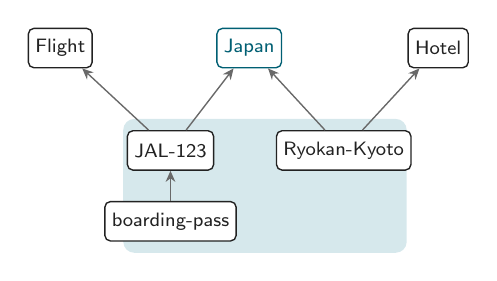
\begin{tikzpicture}[x=1mm, y=1mm]
        \fill[accentlight, rounded corners=4pt] (8,-4) -- (44,-4) -- (44,13) -- (8,13) -- cycle;
        \node[cat] (fl) at (0,22) {Flight};
        \node[cat, draw=accent, text=accent] (ja) at (24,22) {Japan};
        \node[cat] (ho) at (48,22) {Hotel};
        \node[cat] (jal) at (14,9) {JAL-123};
        \node[cat] (ry) at (36,9) {Ryokan-Kyoto};
        \node[cat] (bp) at (14,0) {boarding-pass};
        \foreach \a/\b in {jal/fl, jal/ja, ry/ho, ry/ja, bp/jal} { \draw[sub] (\a) -- (\b); }
      \end{tikzpicture}\par
      \vspace{2mm}
      {\scriptsize\color{soft}the shaded cone is everything below Japan\par}
    \end{column}
  \end{columns}
  \vspace{3mm}
  \small
  \begin{itemize}\setlength{\itemsep}{1.2mm}
    \item \code{put} files a name under its parents; \code{get} returns what lies below every name you give. The boarding pass was never filed under Japan: it is below the flight, which is.
    \item In loopmarket a want's terms are one \code{get}; a give is one of its answers.
  \end{itemize}
\end{frame}

\begin{frame}{Typed values: time, place, mass are categories too}
  \begin{columns}[T]
    \begin{column}{0.52\textwidth}
      {\scriptsize\ttfamily
        \textcolor{soft}{\$} odag put JAL-123 \textquotesingle{}time(2026-07-14)\textquotesingle{}\\[0.4mm]
        \textcolor{soft}{\$} odag get Flight \textquotesingle{}time(2026-06-01..2026-08-31)\textquotesingle{}\\[0.4mm]
        JAL-123\quad boarding-pass\par}
      \vspace{3mm}
      \footnotesize
      \renewcommand{\arraystretch}{1.25}
      \begin{tabular}{@{}l@{\quad}l@{}}
        \code{time(2026-11-06)} & a day: the set of its instants \\
        \code{geo(48.8584,2.2945±500m)} & a square 500\,m either way \\
        \code{mass(..5kg)} & at most 5\,kg \\
        \code{temperature(24C)} & exact, on the kelvin scale \\
      \end{tabular}
    \end{column}
    \begin{column}{0.46\textwidth}
      \centering
      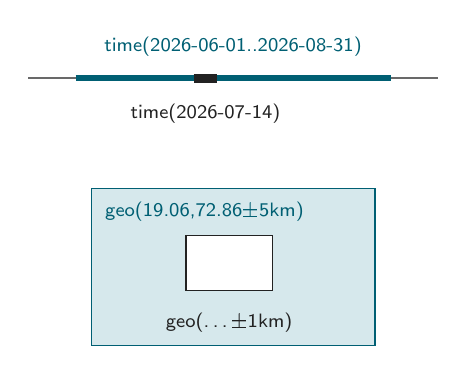
\begin{tikzpicture}[x=1mm, y=1mm]
        \draw[soft] (0,20) -- (52,20);
        \draw[accent, line width=2.2pt] (6,20) -- (46,20);
        \draw[ink, line width=3.2pt] (21,20) -- (24,20);
        \node[font=\scriptsize, text=accent] at (26,24) {time(2026-06-01..2026-08-31)};
        \node[font=\scriptsize] at (22.5,15.5) {time(2026-07-14)};
        \draw[accent, fill=accentlight] (8,-14) rectangle (44,6);
        \draw[ink, fill=white] (20,-7) rectangle (31,0);
        \node[font=\scriptsize, text=accent, anchor=north west] at (8.5,5.5) {geo(19.06,72.86±5km)};
        \node[font=\scriptsize] at (25.5,-11) {geo(…±1km)};
      \end{tikzpicture}
    \end{column}
  \end{columns}
  \vspace{2mm}
  \small
  \begin{itemize}\setlength{\itemsep}{1mm}
    \item A value is a set; one sits below another when its set lies inside the other's. The order is computed from the names, never stored: no edge links 14 July to the summer.
    \item Values are exact rationals of SI units (500\,g is $\frac12$\,kg), so every replica computes the same order. Overlap is a different question: it is not transitive, so it is never \emph{fits within}.
  \end{itemize}
\end{frame}

\begin{frame}{Matching in loopmarket: three relations, one rule}
  \vspace{-1mm}
  \footnotesize
  \renewcommand{\arraystretch}{1.08}
  \begin{tabular}{@{}>{\raggedright\arraybackslash}p{33mm}>{\raggedright\arraybackslash}p{37mm}c>{\raggedright\arraybackslash}p{54mm}@{}}
    \toprule
    \textbf{want} & \textbf{give} & & \textbf{why} \\
    \midrule
    fruit & apple & \tick & meaning: the give lies within the want \\
    apple & fruit & \cross & a fruit might be a banana \\
    within 5\,km of Jio & within 1\,km of Jio & \tick & place: one box contains the other \\
    box A & box B, partly overlapping & \cross & overlap is not containment \\
    Friday 6 November & Friday, 18:00--20:00 & \tick & time: one window contains the other \\
    a bookcase, moved & \code{transport(furniture)} & \tick & an operator's argument: the moved thing lies within it \\
    a piano, moved & \code{transport(furniture)} & \cross & a piano is not furniture \\
    flurb & anything & \cross & an unknown word never matches: it fails closed \\
    \bottomrule
  \end{tabular}
  \vspace{3mm}

  {\small Whoever fixes a value states a fact; whoever leaves it open states what they accept; the fact must lie within the acceptance. Your own places stay private: \code{loop place home 46.05,14.50+-5km} publishes only the box.\par}
\end{frame}

\begin{frame}{A shared catalogue, pinned by every offer}
  \begin{columns}[T]
    \begin{column}{0.49\textwidth}
      \small
      \begin{itemize}\setlength{\itemsep}{2mm}
        \item \textbf{Canonical.} Equal content gives an equal root hash, whoever builds it and in whatever order.
        \item \textbf{Pinned.} Every offer names the catalogue root it was written against. Offers pinned to different roots never pair, so a match is reproducible forever.
        \item \textbf{Verifiable.} An answer that one category lies below another can carry a certificate that anyone checks against the root.
      \end{itemize}
    \end{column}
    \begin{column}{0.49\textwidth}
      \small
      \begin{itemize}\setlength{\itemsep}{2mm}
        \item \textbf{A shared core.} About 4,800 categories in fourteen branches, built by consensus over WordNet, SUMO, OpenCyc, schema.org, YAGO, BFO, DOLCE and Wikidata: each edge carried by two independent sources or an explicit ruling. Ten domain packs add about 6,700 more.
        \item \textbf{On Swarm.} The packs are published there and adopted by fingerprint; adopting one reproduces its root byte for byte.
        \item \textbf{In a browser.} ontodag's own organiser page runs the package in the browser, and is itself a Swarm site.
      \end{itemize}
    \end{column}
  \end{columns}
\end{frame}
}


% ---------------------------------------------------------------- part 4: Swarm and the page

% ================================================================ 7 swarm
\begin{frame}{Swarm: a server nobody owns}
  \vspace{-1mm}
  \footnotesize
  \renewcommand{\arraystretch}{1.2}
  \begin{tabular}{@{}>{\raggedright\arraybackslash}p{57mm}>{\raggedright\arraybackslash}p{78.5mm}@{}}
    \toprule
    \textbf{\color{accent}what Swarm gives} & \textbf{\color{accent}what loopmarket does with it} \\
    \midrule
    \textbf{Content addressing}: data is named by its hash
      & an offer's id is its hash; equal books give equal roots, byte for byte; inclusion proofs are checked on chain \\
    \textbf{Feeds}: mutable pointers, signed by their owner
      & each maker's book is their own feed: identity is a key; no account, no platform \\
    \textbf{Postage}: storage prepaid, no hosting account; it all goes to the node operators
      & a maker pays only for their own book, and reading it costs them nothing \\
    \textbf{Thousands of independent nodes}, permissionless
      & nobody can delist an offer; an aggregator that drops a book is caught by an absence proof \\
    \textbf{Encryption and access control}, client side
      & delivery details are sealed to the counterparty, inside the book \\
    \textbf{Websites are content too}
      & the market page is itself a Swarm site: it folds every book in the browser \\
    \bottomrule
  \end{tabular}
  \vspace{2.5mm}

  On chain only what needs consensus: one announcement per book, the batches, the escrow.
\end{frame}

\begin{frame}{One market from many books: the fold}
  \centering
  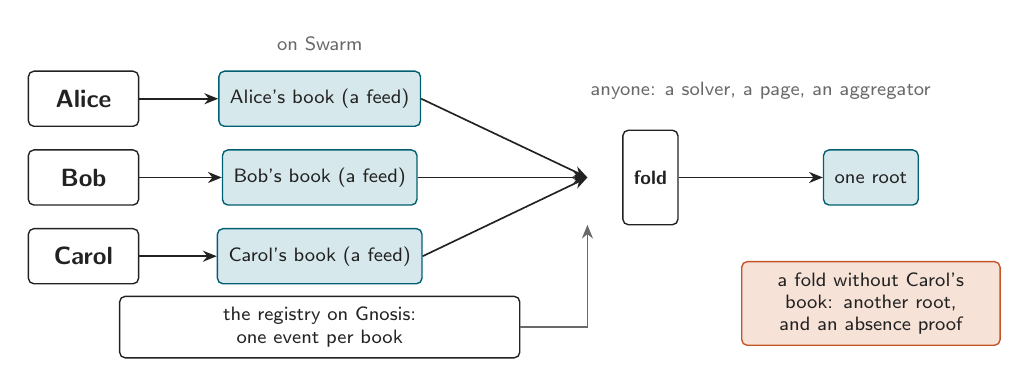
\begin{tikzpicture}[x=1mm,y=1mm]
    \foreach \n/\y in {Alice/10,Bob/0,Carol/-10} {
      \node[maker, minimum width=14mm] (m\n) at (0,\y) {\n};
      \node[box, font=\scriptsize, fill=accentlight, draw=accent] (b\n) at (30,\y) {\n's book (a feed)};
      \draw[flow] (m\n) -- (b\n);
      \draw[flow] (b\n.east) -- (64,0);
    }
    \node[box, font=\scriptsize, text width=48mm] (R) at (30,-19) {the registry on Gnosis:\\ one event per book};
    \draw[flow, soft] (R.east) -| (64,-6);
    \node[box, font=\scriptsize\bfseries, minimum height=12mm] (F) at (72,0) {fold};
    \node[box, font=\scriptsize, fill=accentlight, draw=accent] (Rt) at (100,0) {one root};
    \draw[flow] (F) -- (Rt);
    \node[bad, font=\scriptsize, text width=30mm] (Bad) at (100,-16) {a fold without Carol's book: another root, and an absence proof};
    \node[note, font=\scriptsize] at (30,17) {on Swarm};
    \node[note, font=\scriptsize] at (86,11) {anyone: a solver, a page, an aggregator};
  \end{tikzpicture}\par
  \vspace{2mm}
  \raggedright
  \small
  \begin{itemize}\setlength{\itemsep}{1.2mm}
    \item Each maker writes only their own book and announces it once. Anyone folds the announced books, under fixed rules: forgeries refused, withdrawals kept.
    \item Same books, in any order: the same root. So an aggregator is only a cache.
  \end{itemize}
\end{frame}


\begin{frame}{The market in a browser: a dynamic website on Swarm}
  \centering
  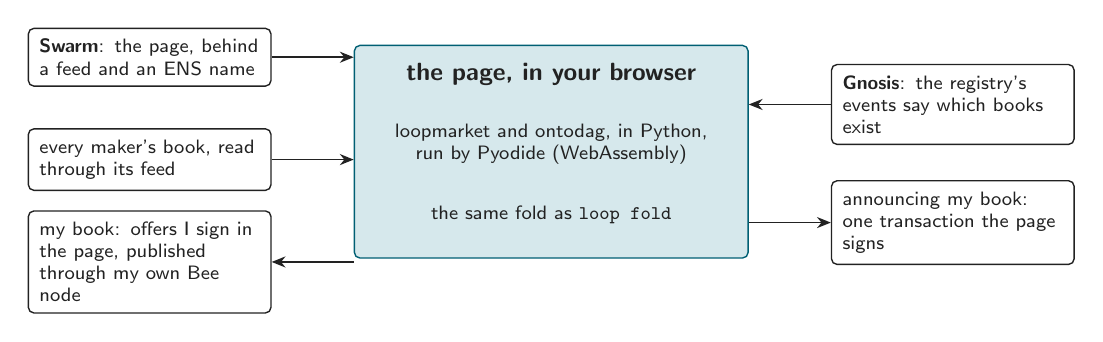
\begin{tikzpicture}[x=1mm,y=1mm,
      side/.style={box, text width=28mm, align=left, font=\scriptsize, execute at begin node={\hyphenpenalty=10000\rightskip=0pt plus 1fil}}]
    \node[box, minimum width=50mm, minimum height=27mm, fill=accentlight, draw=accent] (P) at (0,0) {};
    \node[font=\small\bfseries, anchor=north] at (0,12.5) {the page, in your browser};
    \node[font=\scriptsize, align=center] at (0,1) {loopmarket and ontodag, in Python,\\ run by Pyodide (WebAssembly)};
    \node[font=\scriptsize, align=center] at (0,-8) {the same fold as \code{loop fold}};
    \node[side] (S1) at (-51,12) {\textbf{Swarm}: the page, behind a feed and an ENS name};
    \node[side] (S2) at (-51,-1) {every maker's book, read through its feed};
    \node[side] (S3) at (-51,-14) {my book: offers I sign in the page, published through my own Bee node};
    \node[side] (G1) at (51,6) {\textbf{Gnosis}: the registry's events say which books exist};
    \node[side] (G2) at (51,-9) {announcing my book: one transaction the page signs};
    \draw[flow] (S1.east) -- (P.west |- S1.east);
    \draw[flow] (S2.east) -- (P.west |- S2.east);
    \draw[flow] (P.west |- S3.east) -- (S3.east);
    \draw[flow] (G1.west) -- (P.east |- G1.west);
    \draw[flow] (P.east |- G2.west) -- (G2.west);
  \end{tikzpicture}\par
  \vspace{3mm}
  \raggedright
  \small
  \begin{itemize}\setlength{\itemsep}{1.2mm}
    \item A static page with dynamic data: the market lives in the makers' feeds. A new version of the page moves one feed, and the names stay.
    \item No install and no key to read; through your own Bee node it also publishes your offers. Checked in Chromium, Freedom Browser and on an iPhone.
  \end{itemize}
\end{frame}


% ---------------------------------------------------------------- part 5: clearing and settlement

% ================================================================ 8 lifecycle
\begin{frame}{From offer to delivery}
  \centering
  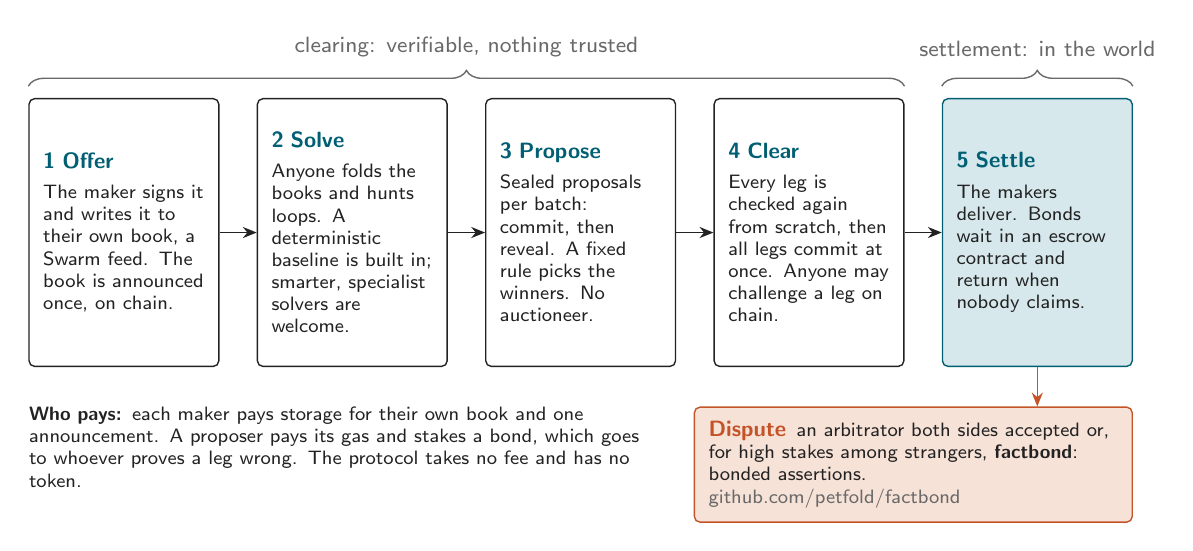
\begin{tikzpicture}[x=1mm, y=1mm,
      nohyph/.style={execute at begin node={\hyphenpenalty=10000\exhyphenpenalty=10000\rightskip=0pt plus 1fil}},
      stage/.style={box, nohyph, text width=20.5mm, minimum height=34mm, align=left, anchor=north, inner sep=1.8mm, font=\scriptsize}]
    \node[stage] (s1) at (0,0)   {{\footnotesize\bfseries\color{accent}1 Offer}\\[1mm]The maker signs it and writes it to their own book, a Swarm feed. The book is announced once, on chain.};
    \node[stage] (s2) at (29,0)  {{\footnotesize\bfseries\color{accent}2 Solve}\\[1mm]Anyone folds the books and hunts loops. A deterministic baseline is built in; smarter, specialist solvers are welcome.};
    \node[stage] (s3) at (58,0)  {{\footnotesize\bfseries\color{accent}3 Propose}\\[1mm]Sealed proposals per batch: commit, then reveal. A fixed rule picks the winners. No auctioneer.};
    \node[stage] (s4) at (87,0)  {{\footnotesize\bfseries\color{accent}4 Clear}\\[1mm]Every leg is checked again from scratch, then all legs commit at once. Anyone may challenge a leg on chain.};
    \node[stage, fill=accentlight, draw=accent] (s5) at (116,0) {{\footnotesize\bfseries\color{accent}5 Settle}\\[1mm]The makers deliver. Bonds wait in an escrow contract and return when nobody claims.};
    \foreach \a/\b in {s1/s2, s2/s3, s3/s4, s4/s5} { \draw[flow] (\a.east) -- (\b.west); }
    \draw[decorate, decoration={brace, amplitude=2mm}, soft] ($(s1.north west)+(0,1.5)$) -- node[note, above=2.5mm] {clearing: verifiable, nothing trusted} ($(s4.north east)+(0,1.5)$);
    \draw[decorate, decoration={brace, amplitude=2mm}, soft] ($(s5.north west)+(0,1.5)$) -- node[note, above=2.5mm] {settlement: in the world} ($(s5.north east)+(0,1.5)$);
    \node[bad, nohyph, text width=52mm, align=left, font=\scriptsize, anchor=north east, inner sep=1.8mm] (d) at ($(s5.south east)+(0,-5)$)
      {{\footnotesize\bfseries\color{warn}Dispute}\enspace an arbitrator both sides accepted or, for high stakes among strangers, \textbf{factbond}: bonded assertions.\\ {\color{soft}github.com/petfold/factbond}};
    \draw[flow, color=warn] (s5.south) -- (s5.south |- d.north);
    \node[nohyph, anchor=north west, text width=80mm, align=left, font=\scriptsize, inner sep=0pt] at ($(s1.south west)+(0,-5)$)
      {\textbf{Who pays:} each maker pays storage for their own book and one announcement. A proposer pays its gas and stakes a bond, which goes to whoever proves a leg wrong. The protocol takes no fee and has no token.};
  \end{tikzpicture}
\end{frame}

\begin{frame}{The sealed batch: competition without an auctioneer}
  \centering
  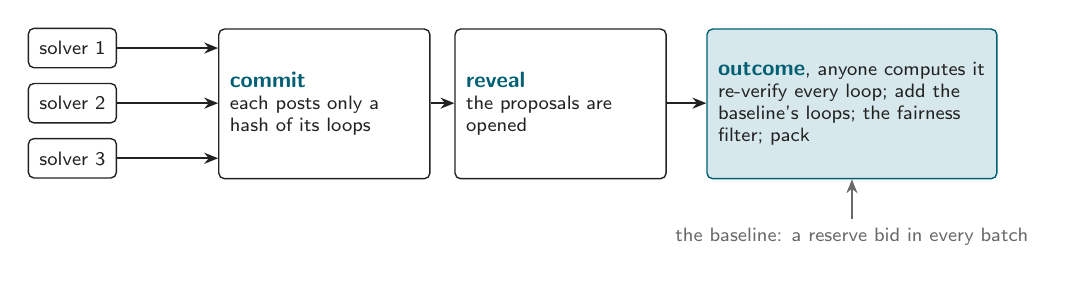
\begin{tikzpicture}[x=1mm,y=1mm,
      st/.style={box, text width=24mm, align=left, font=\scriptsize, minimum height=19mm, anchor=north}]
    \foreach \i/\y in {1/7,2/0,3/-7} { \node[box, font=\scriptsize, minimum height=5mm] (sv\i) at (0,\y) {solver \i}; }
    \node[st] (c) at (32,9.5) {{\footnotesize\bfseries\color{accent}commit}\\ each posts only a hash of its loops};
    \node[st] (r) at (62,9.5) {{\footnotesize\bfseries\color{accent}reveal}\\ the proposals are opened};
    \node[st, text width=34mm, fill=accentlight, draw=accent] (o) at (99,9.5) {{\footnotesize\bfseries\color{accent}outcome}, anyone computes it\\ re-verify every loop; add the baseline's loops; the fairness filter; pack};
    \foreach \i in {1,2,3} { \draw[flow] (sv\i.east) -- (c.west |- sv\i.east); }
    \draw[flow] (c.east |- 0,0) -- (r.west |- 0,0);
    \draw[flow] (r.east |- 0,0) -- (o.west |- 0,0);
    \node[note, font=\scriptsize] (base) at (99,-17) {the baseline: a reserve bid in every batch};
    \draw[flow, soft] (base) -- (o.south);
  \end{tikzpicture}\par
  \vspace{3mm}
  \raggedright
  \small
  \begin{itemize}\setlength{\itemsep}{1.2mm}
    \item Sealed: nobody can copy or front-run a proposal they cannot see. No auctioneer: every replica computes the same winners from the revealed set.
    \item The fairness filter (CoW's CIP-67, generalised to cycles) drops a proposal that leaves an offer worse off than its best alternative; then packing, scored in logs of surplus.
    \item Not built yet: threshold-encrypted sealing, and paying solvers (a spread leg).
  \end{itemize}
\end{frame}


\begin{frame}{Optimistic clearing: why anyone may challenge}
  \centering
  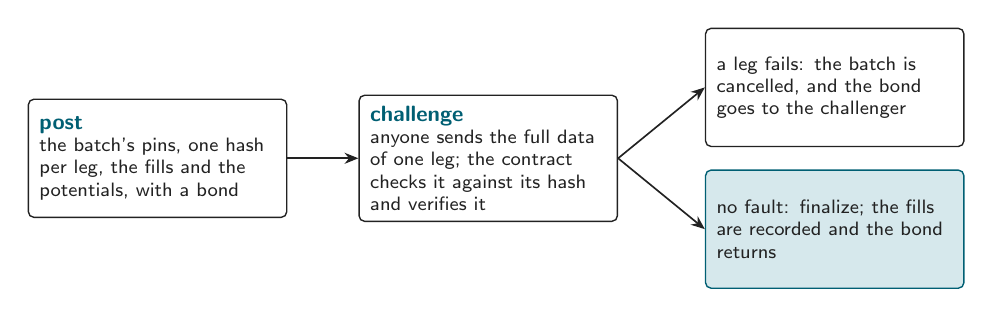
\begin{tikzpicture}[x=1mm,y=1mm,
      st/.style={box, text width=30mm, align=left, font=\scriptsize, minimum height=15mm}]
    \node[st] (s) at (0,0) {{\footnotesize\bfseries\color{accent}post}\\ the batch's pins, one hash per leg, the fills and the potentials, with a bond};
    \node[st] (w) at (42,0) {{\footnotesize\bfseries\color{accent}challenge}\\ anyone sends the full data of one leg; the contract checks it against its hash and verifies it};
    \node[bad, st] (x) at (86,9) {a leg fails: the batch is cancelled, and the bond goes to the challenger};
    \node[st, fill=accentlight, draw=accent] (f) at (86,-9) {no fault: finalize; the fills are recorded and the bond returns};
    \draw[flow] (s) -- (w);
    \draw[flow] (w.east) -- (x.west);
    \draw[flow] (w.east) -- (f.west);
  \end{tikzpicture}\par
  \vspace{3mm}
  \raggedright
  \small
  \begin{itemize}\setlength{\itemsep}{1.2mm}
    \item Why: the offers live on Swarm, and checking every leg on chain would cost far more than recording commitments. The chain checks only what someone disputes; whether a give fits within a want is the arbiter's.
    \item Who: the makers a false batch would bind, rival solvers it blocks, anyone after the bond. Open: challenges are run by hand today, and bonds sized to the damage are not built.
  \end{itemize}
\end{frame}


\begin{frame}{Settlement: delivery, in the world}
  {\color{accent}\bfseries Who pays if it goes wrong, and did they check?\par}
  \vspace{2mm}
  \small
  \begin{itemize}\setlength{\itemsep}{1.6mm}
    \item \textbf{Bonds.} A give can be backed by a bond held in an escrow contract and reserved for each fill. A want can require one (``a no-show costs me 20''), and a bond declared but not deposited matches nothing.
    \item \textbf{Most cases need no ruling.} A reservation returns to the giver after a quiet claim period, or at once on the wanter's countersignature. A giver who cancels pays the amount the wanter's ladder sets for that notice.
    \item \textbf{Disputes} start with a notice and a chance to cure, then go to an arbitrator both sides accepted, whose ruling is final. For high stakes among strangers there is \textbf{factbond}: bonded assertions, a ladder of rulings, deposits forfeited on reversal.
    \item \textbf{Credentials.} A want may require statements from registers it trusts; the counterparty gate fails closed.
  \end{itemize}
  \vspace{1mm}
  {\scriptsize\color{soft}github.com/petfold/factbond\par}
\end{frame}

\begin{frame}{Who pays for what}
  \small
  \renewcommand{\arraystretch}{1.35}
  \begin{tabular}{@{}>{\raggedright\arraybackslash}p{22mm}>{\raggedright\arraybackslash}p{59mm}>{\raggedright\arraybackslash}p{50mm}@{}}
    \toprule
    & \textbf{pays} & \textbf{gets} \\
    \midrule
    maker & storage for their own book; one announcement & the trade, at or better than their own price \\
    solver & the gas to post a proposal, and a bond & designed: a spread leg inside the loop it found \\
    challenger & gas & the bond of a proposal it proves wrong \\
    aggregator & its own storage and bandwidth & paid serving, never paid inclusion \\
    the protocol & \multicolumn{2}{>{\raggedright\arraybackslash}p{113mm}@{}}{\textbf{nothing, either way}: no fee, no token, no rewards. A real loop looks exactly like a wash trade, so any reward tied to volume would pay people to trade with themselves.} \\
    \bottomrule
  \end{tabular}
\end{frame}
\begin{frame}{CoW Protocol and loopmarket}
  \vspace{-1mm}
  \footnotesize
  \renewcommand{\arraystretch}{1.0}
  \begin{tabular}{@{}>{\raggedright\arraybackslash}p{22mm}>{\raggedright\arraybackslash}p{50mm}>{\raggedright\arraybackslash}p{59mm}@{}}
    \toprule
    & \textbf{CoW Protocol} & \textbf{loopmarket} \\
    \midrule
    traded & tokens & anything the catalogue describes, money included \\
    matching & the same two token addresses, a limit price & fits within, in the catalogue: meaning, place, time \\
    unit of price & token amounts, scored in the native token & each maker's own scale; scored in logs, unit-free \\
    intents live in & CoW's order book & each maker's book, a Swarm feed \\
    auctioneer & the autopilot, one per chain & none: sealed batches on chain, a rule anyone recomputes \\
    solvers & bonded and allowlisted & anyone who posts the bond \\
    after the trade & nothing: the tokens arrived & delivery, bonds in escrow, arbitration \\
    \bottomrule
  \end{tabular}
  \vspace{2mm}

  {\small Same family: signed intents, batches, solvers trusted with nothing. Different market: CoW's rings compete with an AMM price, a loop of rides and repairs with no trade at all. The fairness filter is CoW's CIP-67, generalised to cycles.\par}
\end{frame}
% ================================================================ 9 status
{\renewcommand{\footcentre}{\bfseries @petfold}
\begin{frame}{Where it stands: open source, live at test amounts}
  \vspace{-1mm}
  \begin{columns}[T]
    \begin{column}{0.26\textwidth}
      {\small\bfseries\color{accent}loopmarket\par}
      {\scriptsize\color{soft}Python, BSD-3, on PyPI\par}
      \vspace{1.5mm}
      \scriptsize
      \tick\ offers, books on Swarm, the fold, the baseline solver, clearing\\[0.8mm]
      \tick\ on Gnosis: announcements, sealed batches, challengeable clearing, escrow\\[0.8mm]
      \tick\ the \code{loop} command line; the market in a browser\\[0.8mm]
      \todo\ next: paying solvers, privacy, first real users
    \end{column}
    \begin{column}{0.24\textwidth}
      {\small\bfseries\color{accent}ontodag\par}
      {\scriptsize\color{soft}Python, BSD-3, on PyPI\par}
      \vspace{1.5mm}
      \scriptsize
      \tick\ the DAG store, typed values (time, geo, mass, \dots), canonical roots, verifiable answers\\[0.8mm]
      \tick\ core: about 4,800 categories, plus ten domain packs, also on Swarm
    \end{column}
    \begin{column}{0.20\textwidth}
      {\small\bfseries\color{accent}factbond\par}
      {\scriptsize\color{soft}bonded assertions\par}
      \vspace{1.5mm}
      \scriptsize
      \tick\ the assertion contract on Gnosis, the escrow's resolver\\[0.8mm]
      \todo\ next: the scored simulation that gates real stakes
    \end{column}
    \begin{column}{0.24\textwidth}
      \centering
      \qr{23mm}{https://github.com/petfold/loopmarket}\par
      {\tiny github.com/petfold/loopmarket\par}
      \vspace{2mm}
      \qr{16mm}{https://github.com/petfold/ontodag}\par
      {\tiny github.com/petfold/ontodag\par}
    \end{column}
  \end{columns}
  \vspace{3mm}
  \shade{warnlight}{0.975\textwidth}{\small
    \textbf{What stays hard:} oracles for physical delivery\sep private matching (ZK fits-within proofs)\sep wash loops\sep capture of the catalogue\sep books thick enough to close loops}
\end{frame}
}
% ================================================================ backup
\appendix

\begin{frame}{Backup: invariants the tests enforce}
  \begin{columns}[T]
    \begin{column}{0.48\textwidth}
      \small
      \begin{itemize}\setlength{\itemsep}{1.6mm}
        \item[U1] One uniform offer form: a thing against the maker's own scale.
        \item[U2] Offers are immutable canonical values; the id is a hash.
        \item[U3] Clearing trusts no solver: every leg re-derived.
        \item[U4] Solvers work on pinned roots.
        \item[U5] Positive rates only.
      \end{itemize}
    \end{column}
    \begin{column}{0.48\textwidth}
      \small
      \begin{itemize}\setlength{\itemsep}{1.6mm}
        \item[U6] A deterministic baseline solver.
        \item[U7] Vocabulary fails closed.
        \item[U9] Exact rationals in everything clearing re-checks.
        \item[U11] No partially filled loop survives a merge unnoticed.
      \end{itemize}
    \end{column}
  \end{columns}
  \vspace{5mm}
  {\small About 475 tests; the contracts' tests run on a local EVM every night.\par}
\end{frame}


\begin{frame}{Backup: the stack}
  \centering
  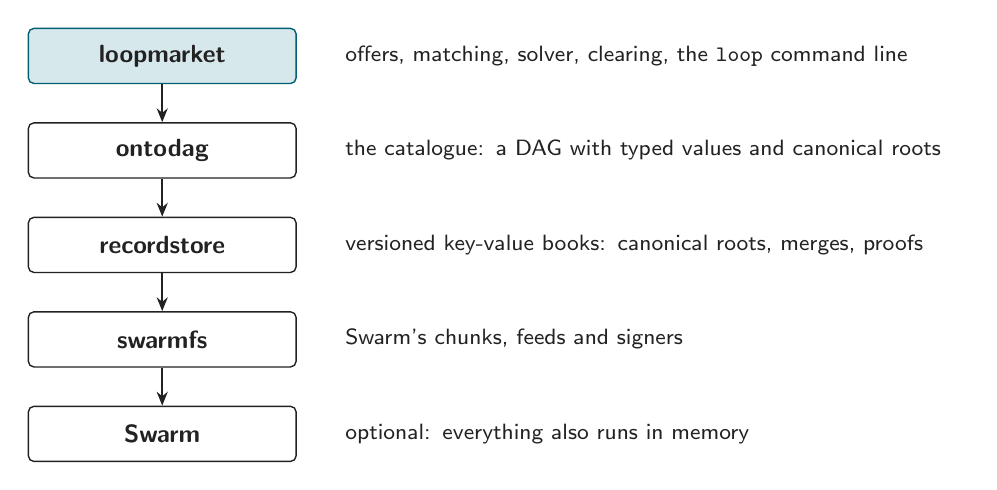
\begin{tikzpicture}[x=1mm,y=1mm, l/.style={box, minimum width=34mm, font=\small\bfseries}, d/.style={anchor=west, font=\footnotesize, text width=78mm}]
    \node[l, fill=accentlight, draw=accent] (lm) at (0,24) {loopmarket};
    \node[l] (od) at (0,12) {ontodag};
    \node[l] (rs) at (0,0) {recordstore};
    \node[l] (sf) at (0,-12) {swarmfs};
    \node[l] (sw) at (0,-24) {Swarm};
    \foreach \a/\b in {lm/od, od/rs, rs/sf, sf/sw} { \draw[flow] (\a) -- (\b); }
    \node[d] at (22,24) {offers, matching, solver, clearing, the \code{loop} command line};
    \node[d] at (22,12) {the catalogue: a DAG with typed values and canonical roots};
    \node[d] at (22,0) {versioned key-value books: canonical roots, merges, proofs};
    \node[d] at (22,-12) {Swarm's chunks, feeds and signers};
    \node[d] at (22,-24) {optional: everything also runs in memory};
  \end{tikzpicture}\par
  \vspace{3mm}
  {\small On Gnosis: the book registry, the beat contract with its leg verifier, the sealed batch, the escrow, and factbond's assertions as the escrow's resolver.\par}
\end{frame}

\end{document}
